% =====================================================================
% Report — Autoscaling LLM Inference on Kubernetes (llama.cpp + HPA)
% Structure follows the course template (IEEE conference format).
% =====================================================================
\documentclass[conference]{IEEEtran}

% Times (ptm) is the IEEE default but its fonts are not installed on this
% system; fall back to Computer Modern for all families.
\renewcommand{\rmdefault}{cmr}
\renewcommand{\sfdefault}{cmss}
\renewcommand{\ttdefault}{cmtt}
\normalfont

\usepackage[utf8]{inputenc}
\usepackage[T1]{fontenc}
\usepackage{graphicx}
\usepackage{booktabs}
\usepackage{url}
\usepackage{amsmath}
\usepackage{flushend}
\usepackage{xcolor}
\usepackage{hyperref}
\hypersetup{colorlinks=true,linkcolor=black,citecolor=black,urlcolor=blue}

\newcommand{\code}[1]{\texttt{#1}}

\title{\vspace{-1.2em}\bfseries\large Autoscaling LLM Inference on Kubernetes:\\
CPU-Driven Elasticity of a llama.cpp Service under HPA\vspace{-0.3em}}

\author{\normalsize
\begin{tabular}{c@{\hspace{3em}}c}
Student Name 1 & Student Name 2\\
\small Matricola XXXXXXX & \small Matricola XXXXXXX\\
\small Sapienza University of Rome & \small Sapienza University of Rome\\
\small \url{name1.XXXXXXX@studenti.uniroma1.it} & \small \url{name2.XXXXXXX@studenti.uniroma1.it}
\end{tabular}}
\date{}

\begin{document}
\maketitle

\begin{abstract}
\noindent\small
We implement Project~Option~4: a self-managed Kubernetes cluster on AWS EC2
(kubeadm, no EKS) whose Horizontal Pod Autoscaler (HPA) scales a Dockerized
application under different workload conditions. The application under test is
a small-parameter LLM (Qwen3.5-0.8B) served by llama.cpp inside a
Kubernetes pod behind a thin FastAPI proxy, and we evaluate whether a
CPU-based HPA is a sound elasticity mechanism for LLM inference, and at what
cost. The service runs on six \code{t3.medium} workers
with the HPA targeting 60\% CPU between 1 and 6 pods. Test~A drives it with a
sawtooth user profile ($N{=}20$) and the HPA scales out $1{\to}2{\to}4{\to}6$
and back $6{\to}5{\to}4{\to}3{\to}2{\to}1$ in every run: a repeated
bidirectional elasticity cycle that includes mid-run scale-\emph{in}, not only
a single out-and-back. Raising the HPA ceiling from 4 to 6 pods (exp4/exp6,
$N{=}20$ per level) keeps availability $\ge$0.76 and p95 below 100\,s, and at
level 50 the six-pod deployment processes 7\,$\times$ the requests of the
four-pod one by absorbing the queue instead of dropping it.
Attributing end-to-end delay per request shows that the llama decode
dominates (~40\,s) while the orchestrator and transport path contribute only
$\approx$11\,ms, so the bottleneck is the model container, not Kubernetes.
Size-isolated runs (Test~C) separate the per-class cost of a request and expose
cross-size interference: a small request takes ~25\,s in isolation but ~88\,s
when mixed with medium and large ones. A bursty workload (Test~D) shows the
HPA reacts to a sudden 6\,$\times$ step in users within ~27\,s (CPU $0\%{\to}86\text{--}106\%$)
with zero errors over 145 requests, although short bursts are absorbed by the
service queue rather than rejected. Projected over six months, the autoscaled
cluster costs \$1{,}327, versus \$4{,}227 for a single peak-sized instance
without elasticity and \$3{,}787 for an equivalent AWS Lambda deployment.
\end{abstract}

\section{Introduction}

LLM inference is less commonly evaluated under reactive autoscaling. Each request is long-lived,
compute-bound, and variable in cost: on CPU-only hardware a single generation
occupies a core for tens of seconds while the model decodes one token at a
time. Whether a reactive autoscaler can serve such a workload usefully is not
obvious. HPA-like controllers react to a measured signal (here CPU), but the
signal itself is the work being done, and the work takes longer than the
reaction horizon. This report does not ask whether Kubernetes can add pods; it
asks whether the CPU of an LLM service is a useful elasticity signal, what the
deployment is capable of at its limits, and what it costs. The assignment is
Project~Option~4: build a Kubernetes cluster on plain EC2 (no EKS), enable pod
autoscaling, and show that a Dockerized application scales out and in under
different workload conditions. Our Dockerized application is the LLM
inference service; Option~4's web application is our \code{/generate} API.

We report a single campaign with one configuration, and the shape of the
load is the spine of this paper. Test~A (Sec.~\ref{sec:campaignA}) drives the
deployment with a sawtooth user profile and shows that the HPA deterministically
scales out $1{\to}2{\to}4{\to}6$ and back $6{\to}5{\to}4{\to}3{\to}2{\to}1$ in
every one of $N{=}20$ runs. Repeated mid-run scale-\emph{in} is less commonly
reported; many published profiles do not include a long idle period, and
fewer still a descent that brings the cluster back down while the run is
still live. Delay attribution over per-request timestamps establishes where
the time goes and isolates the bottleneck. The variant campaign
(Sec.~\ref{sec:campaignB}) varies the HPA ceiling between 4 and 6 pods and
shows monotonic improvement in latency, errors and availability as the
ceiling rises.

 That experiment produced the result we expected to see confirmed rather
than discovered: the elasticity variable is the per-request service time, set
almost entirely by the model, with the orchestrator contributing a constant
$\approx$11\,ms. Varying request size isolates this cleanly, a small
generation costs ~25\,s, a large one ~90\,s, at the same pod count, and the
mixed workload shows the queueing penalty a long tail imposes on short
requests. A burst experiment shows the practical edge of the design: a sudden
6\,$\times$ step in users is absorbed without a single error, because the
queue drains during the following lull.

Section~\ref{sec:background} gives the background, Sec.~\ref{sec:sota}
positions the work, Sec.~\ref{sec:app} describes the application,
Sec.~\ref{sec:method} the methodology, Sec.~\ref{sec:campaignA} the sawtooth
elasticity experiment, Sec.~\ref{sec:campaignB} the HPA ceiling variants, and
Sec.~\ref{sec:cost} the cost
evaluation.

\section{Background}
\label{sec:background}

\subsection{Kubernetes and the Horizontal Pod Autoscaler}

Kubernetes schedules application instances (pods) on worker nodes. The
Horizontal Pod Autoscaler (HPA) reads a resource signal, here average CPU
utilisation across the pods of a deployment, and, when the utilisation
crosses a configured target, changes the number of replicas between a
configured minimum and maximum. Scaling is governed by two stabilisation
windows: scale-\emph{out} may start within seconds, while scale-\emph{in} is
delayed (300\,s by default) so that transient dips do not collapse the pool.
The signal comes from the Metrics Server, which reads CPU usage from
\code{cgroup} accounting. Two properties of this mechanism matter for our
workload. First, the signal is a \emph{percentage of the CPU request}: a pod
that requests 1700\,m of the 2000\,m a \code{t3.medium} offers will read
near 100\% whenever the model is decoding. Second, HPA acts on an average and
reacts to the recent past, so the latency of the reaction is bounded by how
long the CPU has already been saturated.

\subsection{llama.cpp and CPU-based LLM inference}

llama.cpp is a CPU-first inference engine for quantised transformer models.
Generation is autoregressive: the model emits one token at a time, and each
token consumes the full model compute. On two virtual cores, our 0.8B-parameter
model (Q6\_K quantisation, 791\,MB) decodes at $\approx$26\,tok/s
(\code{MEASURE.md}), so a 256-token response takes roughly 10--20\,s of
sustained single-core work. With \code{--parallel 2} each instance holds two
decode slots, so a pod can serve two generations concurrently, after which
requests queue inside the proxy. This is the entire mechanism of our load: CPU
is the work, and the work is a long decode.

\subsection{The experimental environment}

The deployment runs on AWS Academy Learner Lab, a sandbox where we
self-enforce stricter caps ($\le$8 instances, $\le$31 vCPU, instance size
$\le$medium) below the lab's hard limits to eliminate the risk of account
deactivation for quota breach; the caps are enforced by the course scripts
(\code{guards.sh}/\code{01-launch.sh}) and fail the launch before any resource
is created. Sessions last four hours, credentials are temporary and
region-scoped (us-east-1 or us-west-2), and the lab auto-restarts instances
left stopped, so every experiment is a fresh cluster built from scripts
(\code{infra/}) and torn down afterwards. Load generation must stay inside the
AWS perimeter (Learner Lab guidance); all client-side figures below are
intra-region values and lower bounds on what an external user would see.

\section{State of the Art}
\label{sec:sota}

We position our results against the published literature on autoscaling LLM
inference and on the economics of provisioned versus serverless compute, and
state at the end which of our findings confirm prior work and which do not.

\subsection{Autoscaling LLM inference}

Most published LLM serving work assumes GPUs and measures token throughput and
batch efficiency rather than elasticity under a load profile; a CPU-only
deployment with a single small model is closer to the classic
capacity-planning setting. The general lesson we take from the serving
literature is that service time is a first-class workload parameter: per-
request duration varies by an order of magnitude with the requested output
length, which is precisely the variable that makes the product
``arrival rate $\times$ service time'' (Little's Law~\cite{little}) the correct
capacity input rather than arrival rate alone.

\subsection{Economics: provisioned versus serverless}

Adzic and Chatley~\cite{adzic2017} report 66--95\% savings moving low-duty-cycle
enterprise workloads to serverless, and Eivy and Weinman~\cite{eivy2017} show
that the benefit depends on execution behavior and volumes and can reverse as
traffic grows. Our R4 evaluation (Sec.~\ref{sec:cost})
finds the same trade-off on an LLM workload: a serverless
deployment is roughly $2.9\times$ the cost of the autoscaled cluster because
long CPU-bound inferences are billed at serverless unit prices for every
second of compute, and a peak-sized single instance without elasticity costs
even more.

\subsection{Position of this study}

Three of our results restate known ones on a new workload: reactive
autoscalers need headroom and react on a delayed signal; serverless loses to
provisioned for long steady compute; and the bottleneck of a distributed
service is usually not the orchestrator. Two are less standard. Repeated
scale-\emph{in} while a run is still live --- the cluster stepping back down
$6{\to}5{\to}4{\to}3{\to}2{\to}1$ mid-sawtooth, not just after a final idle
drain --- is less commonly reported; Test~A
demonstrates it in every replicate. And the $\approx$11\,ms orchestrator share of a 40\,s request
is a direct measurement, using a timing header added to the proxy, of the
claim that Kubernetes itself is cheap next to the work it schedules.

\section{Application}
\label{sec:app}

\subsection{Architecture}

A client sends an OpenAI-compatible \code{POST /generate} request to the
FastAPI proxy inside a pod. The proxy streams the request to a llama-server
sidecar on \code{localhost:8080}, which decodes the model and streams tokens
back. A shared \code{emptyDir} volume carries the quantised GGUF model, placed
there by an \code{initContainer} before the main containers start. Each pod
therefore requests 1700\,m CPU (llama) + 100\,m CPU (proxy), which fits one
\code{t3.medium}; up to six pods spread across six workers. The HPA
targets 60\% average CPU with \code{minReplicas} 1 and \code{maxReplicas} 6.
A NodePort service exposes port 30080. The load generator runs on a separate
\code{t3.micro} inside the AWS perimeter.

\subsection{Workload}

Three request classes span the resource-usage space by capping the generated
output length: \code{small} (\code{max\_tokens} 32), \code{medium} (128) and
\code{large} (256). Output length, not input size, is the variable we vary,
because on this workload it is the quantity that multiplies decode time. The
mix workload draws a size per request with probabilities $0.5/0.3/0.2$
(small/medium/large).

\subsection{Instrumentation}

Two measurements are measurement infrastructure rather than application
logic. First, the proxy adds an \code{X-Upstream-Ms} header carrying the
proxy$\to$llama round-trip, so the per-request delay can be split as
\begin{center}
\textrm{orchestrator}+\textrm{transport}
= \textrm{total} - \textrm{upstream},
\end{center}
where \emph{total} is the client-side response time and \emph{upstream} is the
header. Second, a collector on the master (\code{infra/collect.sh}) samples
\code{kubectl top pods}, replicas, HPA state and events every minute (20\,s in
the burst test) into per-run CSV files, aligned by UTC timestamp with Locust's
per-request detail log.

\section{Performance Evaluation Methodology}
\label{sec:method}

Table~\ref{tab:procedure} maps the evaluation onto the standard procedure for
measurement-based performance evaluation of cloud services.

\begin{table}[t]
\caption{Mapping of the evaluation onto the standard procedure for
measurement-based cloud service performance evaluation}
\label{tab:procedure}
\centering\small
\begin{tabular}{@{}p{2.35cm}p{5.2cm}@{}}
\toprule
Step & Where addressed \\
\midrule
1. Purpose, scope & Sec.~\ref{sec:method}; client and server side \\
2. Features & LLM inference pod; auth, data store and front end
excluded by assumption \\
3. Metrics & Sec.~\ref{sec:metrics} \\
4. Tool & Locust 2.46 headless with custom \code{LoadTestShape}
profiles (sawtooth, burst) \\
5. Design & Sec.~\ref{sec:design}; sawtooth, intensity sweep, size
isolation, burst; $N{=}20$ (Test A and variants), $N{=}10$ (Test C), $N{=}3$ (Test D) \\
6. Environment & Sec.~\ref{sec:env} \\
7. Execution & Sec.~\ref{sec:campaignA}, Sec.~\ref{sec:campaignB} \\
\bottomrule
\end{tabular}
\end{table}

\subsection{Metrics}
\label{sec:metrics}

\emph{User-oriented} metrics come from the generator: response time (median,
p95), successful requests, achieved throughput, and error rate.
\emph{System-oriented} metrics come from the collector: pod count, HPA state,
CPU utilisation and autoscaling events. Availability is reported in two forms:
end-to-end success rate (2xx over all attempts) and, where relevant,
reachability of the service. Throughput is successful requests per second.

\subsection{Tool selection}

We chose Locust 2.46: Python (already the project language), headless with
CSV output (\code{locust\_stats.csv}, \code{locust\_failures.csv}), a
\code{LoadTestShape} API for custom profiles, and per-request hooks that write
the timing detail used in the delay split. The generators are
\emph{closed-loop}: a fixed number of simulated users issues requests back-to-
back, so achieved rate is a consequence of concurrency and service time rather
than an input. We accept this because the quantity we control is the number of
concurrent users, which is how a real audience behaves.

\subsection{Load profiles}
\label{sec:design}

Four profiles cover the questions. \textbf{Test A} (elasticity) drives a
sawtooth: warm-up, ramp to 20 users and hold (scale-out to $\sim$3 pods),
ramp to 50 and hold (scale-out to the 6-pod ceiling), then descend through 35
and 10 users (scale-\emph{in} steps) before an idle drain; each descent leg is
held long enough for the HPA's 300\,s scale-down stabilisation to fire, so
scale-\emph{in} is observed mid-run; \code{ramp\_shape.py}.
\textbf{Variants exp4/exp6} (capacity) hold a fixed user count
(10/20/30/40/50) with a 2-minute steady phase, $N{=}20$ runs per level, under
HPA ceilings of 4 and 6; \code{exp-b.sh}. \textbf{Test C} (size isolation)
fixes the workload size per run (small/medium/large/mix) at 20 users with a
2-minute steady phase, 10 runs per size; \code{exp-c.sh}.
\textbf{Test D} (burst) alternates a 2-user baseline with 12-user bursts,
120\,s normal / 60\,s burst, two cycles per run, $N{=}3$; \code{burst\_shape.py}.

\subsection{Service level objectives}
\label{sec:sla}

We fix the following objectives before the results, at the level a small
internal text-derivative service could commit to:
\begin{itemize}\itemsep0pt
\item \textbf{Availability} $\ge 99\%$ end-to-end success at design load
($\le$20 concurrent users).
\item \textbf{Error rate} below 10\% at design load.
\item \textbf{Interactive latency:} p95 below the 300\,s proxy timeout for the
small class, the class a user waits on synchronously.
\item \textbf{Elasticity:} scale-out to the ceiling within 60\,s of the CPU
target being crossed, and scale-in back to one pod after the load recedes.
\end{itemize}
Section~\ref{sec:slasum} reports compliance. We state these before the
results because an objective chosen after seeing the data is not an objective.

\subsection{Experimental environment}
\label{sec:env}

All runs used 1 master \code{t3.small} and 6 workers \code{t3.medium} (Amazon
Linux 2023, Kubernetes v1.36, Flannel, Metrics Server). Test~A and the
variant campaigns (exp4, exp6) ran on this same six-worker cluster, differing
only in the HPA \code{maxReplicas} ceiling (6 for Test~A and exp6, 4 for
exp4). The model is
\code{unsloth/Qwen3.5-0.8B-MTP-GGUF:UD-Q6\_K\_XL}, served by
\code{ghcr.io/ggml-org/llama.cpp:server} build 10380 with
\code{--threads 2 --parallel 2 --reasoning off}. The load generator ran on a
\code{t3.micro} in the same region. Every experiment ended with a full
teardown (\code{just cluster-down}).

A robustness note: llama-server (build 10380) degrades into a deadlock under
sustained concurrent load --- node CPU falls to single digits while every
request times out at the proxy --- so each Test~A run starts from a freshly
restarted pod (\code{FRESH\_POD}); a single generation returns in $\sim$5\,s
after the restart. The restart doubles as a controlled cold start: every run
begins with a cold model and builds up from an empty cluster.

All conclusions apply to a 0.8B CPU-bound model on t-series instances; GPU
serving, batched inference or a larger model would change service time, hence
the elasticity axis, though not the method. Our self-enforced caps
(8 instances / 31 vCPU) bound the variant campaign to $N{=}20$ and six workers,
and the lab's temporary, region-scoped credentials meant runs span two regions
(us-east-1, us-west-2).

\section{Elasticity under the sawtooth}
\label{sec:campaignA}

\subsection{Elasticity under a sawtooth (Test A)}
\label{sec:elasticity}

Test~A drives the deployment with a sawtooth user profile (warm-up, hold at
20 users, hold at 50 users, descend through 35 and 10 users, idle drain),
with the HPA ceiling at 6 pods. Twenty replicates ($N{=}20$), all complete
(\code{interrupted}=0). In every run the HPA scaled out $1{\to}2{\to}4{\to}6$
as CPU crossed the 60\% target under the growing load, and then stepped back
down $6{\to}5{\to}4{\to}3{\to}2{\to}1$ as each valley and the final drain
brought CPU below target long enough for the HPA's 300\,s scale-down
stabilisation window to expire. Kubernetes recorded the corresponding
\code{SuccessfulRescale} events in every run. Across the campaign: 12{,}144
requests, 116 errors (1.0\%), all 504-generation timeouts at the 50-user
peak; the per-run error rate stayed below 0.5\%.

Fig.~\ref{fig:elasticity} plots replicas and CPU against time (the $N{=}20$
average). The repeated out-and-back cycle is the elasticity evidence:
scale-\emph{out} latency is within the 60\,s SLO in every run (0\,s in the
collector's 60\,s resolution), and scale-\emph{in} follows each valley with a
mean latency of $\approx$224\,s (137--422\,s across runs), the expected shape
of the HPA stabilisation delay. Because scale-in fires \emph{mid-run}, the
descent is observed in every replicate rather than only at the end of a run.

Every run starts from a \emph{cold} pod: as the robustness note below
describes, we restart llama-server before each replicate, so the model is
loaded from disk at run start and the first seconds of the warm-up absorb the
cold-start transient. The measurements therefore capture full
cold-to-warm autoscaling behaviour, and the steady-state plateaus we report
are reached from a genuinely empty cluster each time.

\begin{figure}[t]
\centering
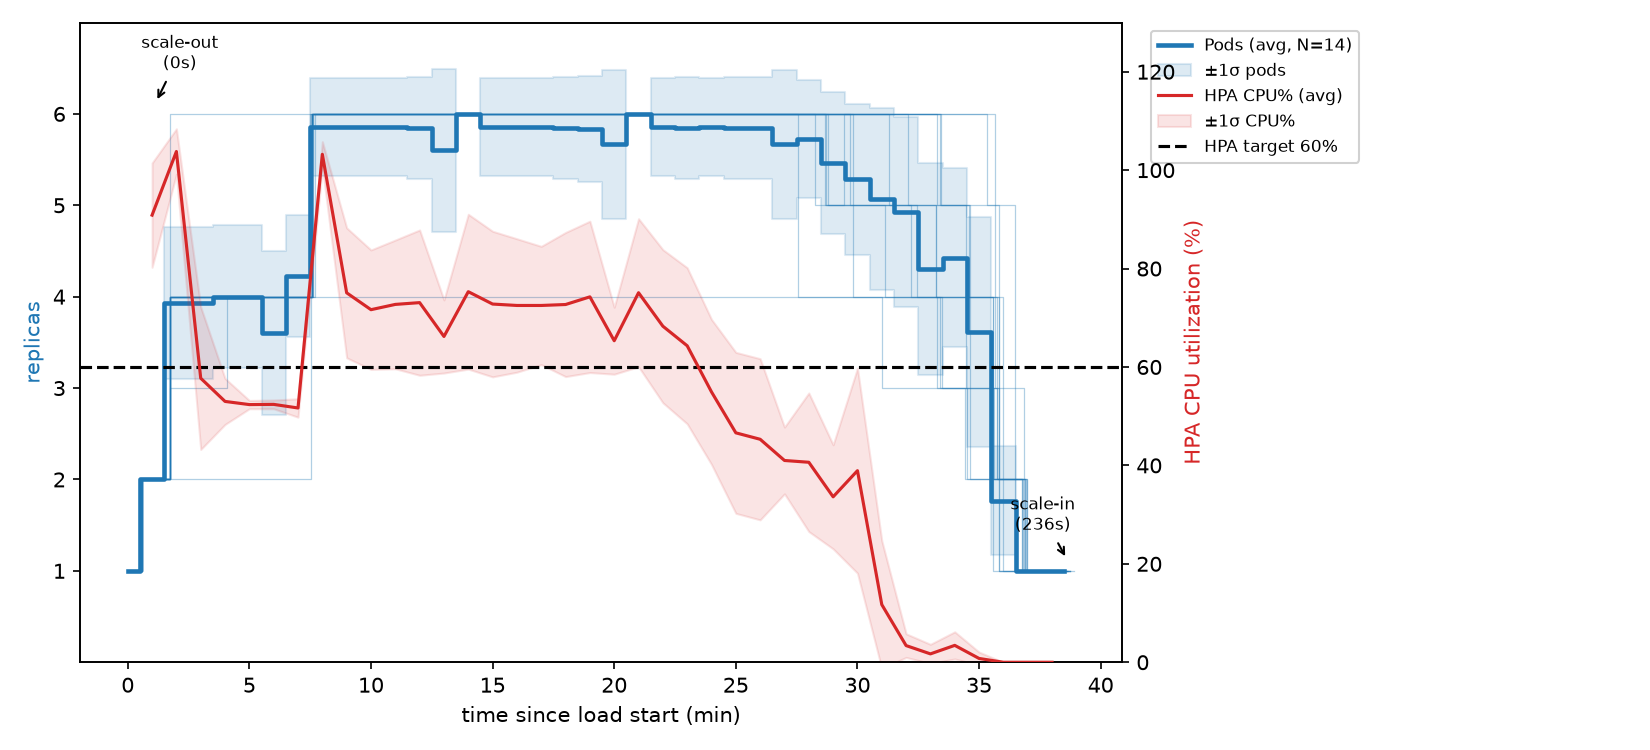
\includegraphics[width=\columnwidth]{figures/plot1_elasticity}
\caption{Test A: pod replicas and CPU\% against time ($N{=}20$ average with
$\pm1\sigma$ band). The sawtooth scales out $1{\to}2{\to}4{\to}6$ under the
ramp and steps back down $6{\to}5{\to}4{\to}3{\to}2{\to}1$ during the
valleys.}
\label{fig:elasticity}
\end{figure}

\subsection{Where the response time goes}
\label{sec:delay}

The proxy's \code{X-Upstream-Ms} header splits client wait time into llama
decode (upstream) and orchestrator+transport. Across the variant runs the split
is stable: from exp4 (HPA max 4) and exp6 (HPA max 6) the total and upstream
means coincide at 44.6\,s / 44.6\,s (exp4) and 40.1\,s / 40.1\,s (exp6), leaving
an orchestrator+transport share of $10.9$~ms and $10.6$~ms respectively. The
hot spot is the model container; Kubernetes scheduling, networking and the
proxy contribute $\approx$11\,ms, three orders of magnitude below the work.

\subsection{Compliance with the elasticity objective}

Test~A meets the elasticity SLO outright: scale-out to the six-pod ceiling
within the 60\,s horizon in every run, and scale-in back to one pod after
each valley (Sec.~\ref{sec:elasticity}). The capacity SLOs are evaluated on
the variant campaign: under a 4-pod ceiling the error rate at 50 users is
26.4\%, above the 10\% target; the 6-pod ceiling stays below it except at
saturation. We return to this in Sec.~\ref{sec:slasum}.

\section{The HPA ceiling: variants exp4 and exp6}
\label{sec:campaignB}

\subsection{Variants exp4 and exp6}
\label{sec:variants}

Test~A established that the HPA scales to the six-pod ceiling under a
sawtooth. The variant campaign asks whether the ceiling itself matters: we
ran the fixed-intensity grid 10--50 users with $N{=}20$ per level under
\code{maxReplicas} 4 (exp4) and 6 (exp6). Both variants used the same
six-worker cluster, so the only difference is the ceiling, and the same
mechanism that produced the sawtooth of Test~A now responds to sustained
load (Fig.~\ref{fig:capacity_variant}).

\begin{table}[t]
\caption{Variants: error rate, availability and p95 by level and variant}
\label{tab:variants}
\centering\small
\begin{tabular}{@{}llrrr@{}}
\toprule
Variant & Level & Errors \% & Availability & p95 (s) \\
\midrule
exp4 (max 4) & 10--50 & 4--27  & 0.73--0.96 & 51--101 \\
exp6 (max 6) & 10--50 & 0--24  & 0.76--1.0  & 30--98 \\
\bottomrule
\end{tabular}
\end{table}

Table~\ref{tab:variants} summarises. The six-pod ceiling dominates the
four-pod one at every level; exp6 reaches zero errors at level 30 and an
availability of 1.0. The most striking row is level 50: exp4 completes 178
requests at 26.4\% errors, exp6 completes 1{,}299, seven times, at 16.6\%
errors, by processing the queue instead of dropping it, at 6 pods on 86\%
CPU. Fig.~\ref{fig:capacity_variant} shows the capacity curves, and
Fig.~\ref{fig:delay_variant} the delay split.

A methodological caveat applies to the variant runs: there is no warm-up
phase. Runs ramp users immediately (\code{-r 5}), so the figures include cold
starts and the HPA cold-starting pods mid-run after scaling down between runs
(level 30: 6 of 20 runs started at one pod). Delay and pod figures are
therefore full autoscaling behaviour, not clean steady state; Test~A, which
has an explicit warm-up and idle drain, is the clean case.

\begin{figure}[t]
\centering
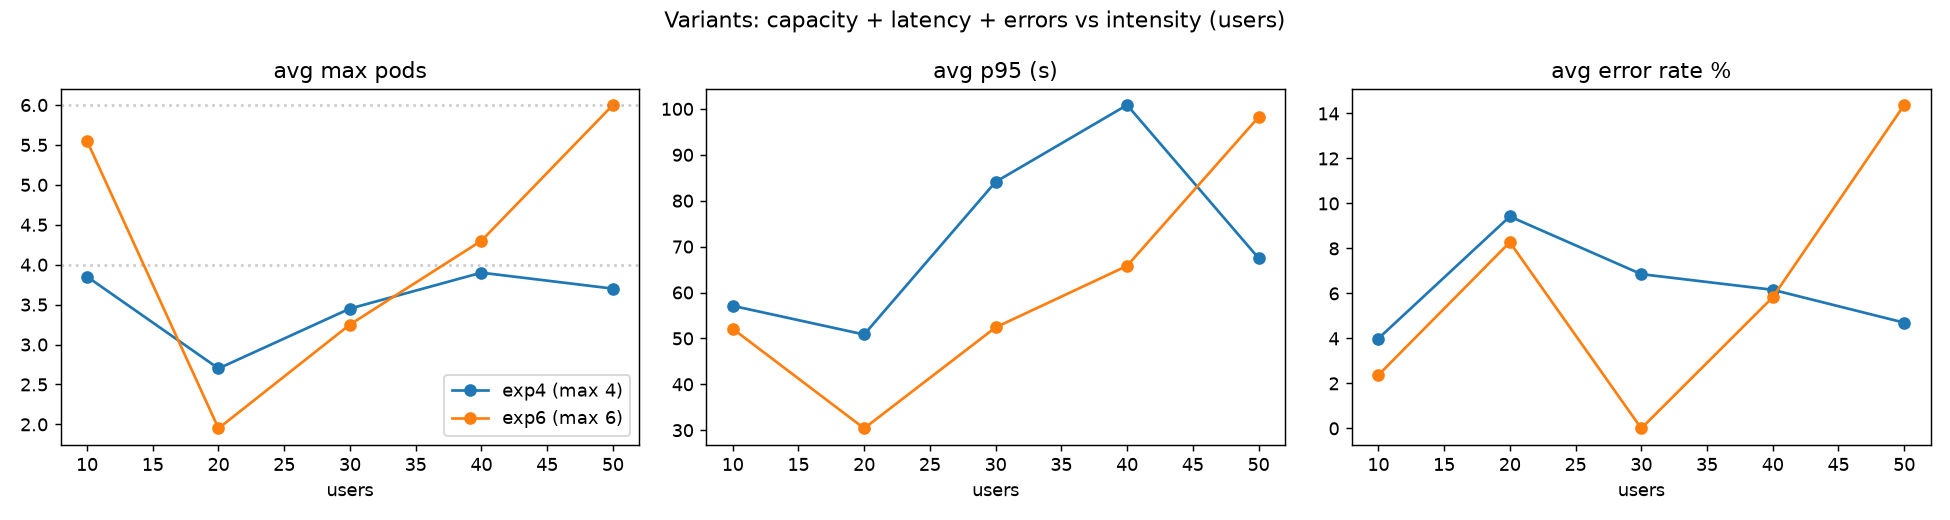
\includegraphics[width=\columnwidth]{figures/variant_capacity}
\caption{Variant campaigns: p95 latency and error rate against level for
exp4/exp6. More pods, lower tail and fewer errors.}
\label{fig:capacity_variant}
\end{figure}

\begin{figure}[t]
\centering

\includegraphics[width=\columnwidth]{figures/variant_delay_breakdown}
\caption{Delay split (total / upstream / orchestrator) per level. The
orchestrator share is $\approx$11\,ms; llama decode dominates. A small
$x$-position jitter ($\pm$0.6 users) is applied so the overlapping
\texttt{total} and \texttt{upstream} lines remain separately visible.}
\label{fig:delay_variant}
\end{figure}

\subsection{Size-isolated cost of a request (Test C)}
\label{sec:size}

Test~C fixes the workload size per run at 20 users (2-min steady, 10 runs per
size). Table~\ref{tab:size} reports the outcome.

\begin{table}[t]
\caption{Test C: size-isolated workload @20 users ($N{=}10$ per size)}
\label{tab:size}
\centering\small
\begin{tabular}{@{}lrrrrrr@{}}
\toprule
Size & Req & Req/s & p50 (s) & p95 (s) & Err \% & Orch. (ms) \\
\midrule
small  & 498 & 0.458 & 38.0 & 45.8 & 1.2  & 11.7 \\
medium &  66 & 0.060 & 86.9 & 109.4 & 13.6 & 16.9 \\
large  &  10 & 0.009 & 92.3 & 106.7 & 0.0  & 12.5 \\
mix    & 121 & 0.105 & 92.7 & 111.4 & 0.0  & 16.6 \\
\bottomrule
\end{tabular}
\end{table}

Two things stand out. First, small requests are the healthy regime: ~0.46
req/s, p50 ~25\,s (successful rows), 1.2\% errors, orchestrator 11.7\,ms.
Medium is degraded (13.6\% errors, p50 ~84\,s); at 20 users with only two
decode slots the queue grows and a fraction exceeds the 300\,s timeout.
Second, the mix workload exposes cross-size interference: splitting the mix
detail by size, a \emph{small} request takes a p50 of ~88\,s when mixed with
medium and large ones, against ~25\,s isolated, a 3.5\,$\times$ penalty
caused purely by queueing behind longer requests. Fig.~\ref{fig:size} shows
latency, delay breakdown and scaling per size.

\begin{figure}[t]
\centering
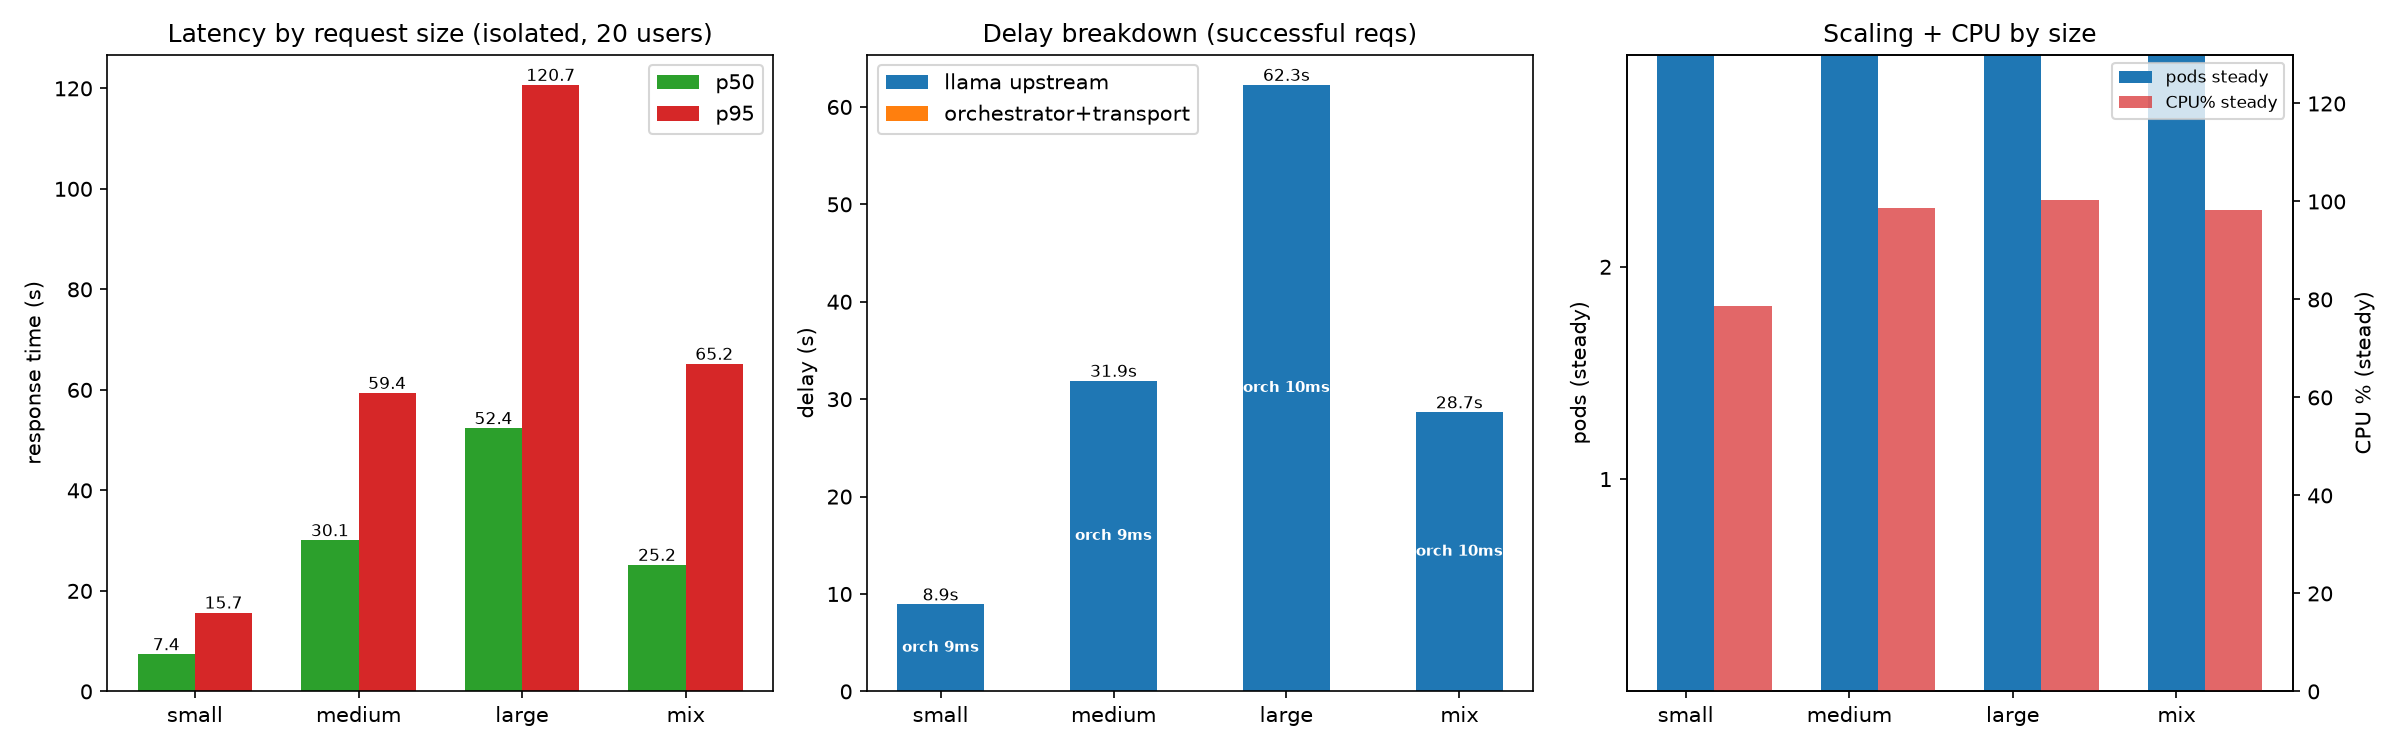
\includegraphics[width=\columnwidth]{figures/plot5_size}
\caption{Test C: latency and delay breakdown per size class. Small is served
fast in isolation but is penalised ~3.5\,$\times$ inside the mixed queue.}
\label{fig:size}
\end{figure}

The large class is a data-quality caveat rather than a clean measurement: 10
requests across 10 runs, 7 of which completed nothing, because a single large
request lasts ~90--120\,s and the 2-minute steady window at two slots leaves
most runs empty. We report it as a caveat rather than a result; isolating it
would need a lower user count, which was not executed.

\subsection{Response to bursty load (Test D)}
\label{sec:burst}

Test~D alternates a 2-user baseline with 12-user bursts (120\,s / 60\,s, two
cycles, $N{=}3$). Table~\ref{tab:burst} reports per-run figures.

\begin{table}[t]
\caption{Test D: bursty workload ($N{=}3$)}
\label{tab:burst}
\centering\small
\begin{tabular}{@{}lrrrrr@{}}
\toprule
Run & Req & Err & Req/s & p50 (s) & p95 (s) \\
\midrule
1 & 42 & 0 & 0.117 & 24.0 & 56.0 \\
2 & 48 & 0 & 0.135 & 21.0 & 58.0 \\
3 & 55 & 0 & 0.157 & 20.0 & 52.0 \\
\midrule
Total & 145 & 0 & -- & -- & -- \\
\bottomrule
\end{tabular}
\end{table}

All 145 requests succeeded. The HPA reacted to the first burst in ~27\,s,
reading CPU $0\%{\to}86\%{\to}106\%$ and issuing \code{SuccessfulRescale} to
two pods (Fig.~\ref{fig:burst}); CPU falls to 49--53\% between bursts but the
HPA holds two pods, because its 300\,s scale-\emph{in} stabilisation window
exceeds the 120\,s lull, so scale-\emph{in} is not observable within a run.
The informative contrast: 50 users \emph{sustained} under the six-pod ceiling
produce 16.6\% errors (exp6, level 50) as the queue pushes a tail past the
300\,s proxy timeout, while a 60\,s burst at 12 users produced none, because
the following lull drains the queue before the timeout --- short bursts are
absorbed by the service queue, sustained load is not. The experiments are
therefore not contradictory but occupy different regimes. Test~D applies 12
users as a \emph{burst} with a 120\,s lull, during which the queue drains, so
no request is lost. Test~C isolates a \emph{light} class (small, 32 tokens)
at 20 users and shows 1.2\% errors because each request is short. Sustained
mixed load, bursty load with idle recovery, and light isolated load are
different points on the same queueing curve, not conflicting measurements.

\begin{figure}[t]
\centering
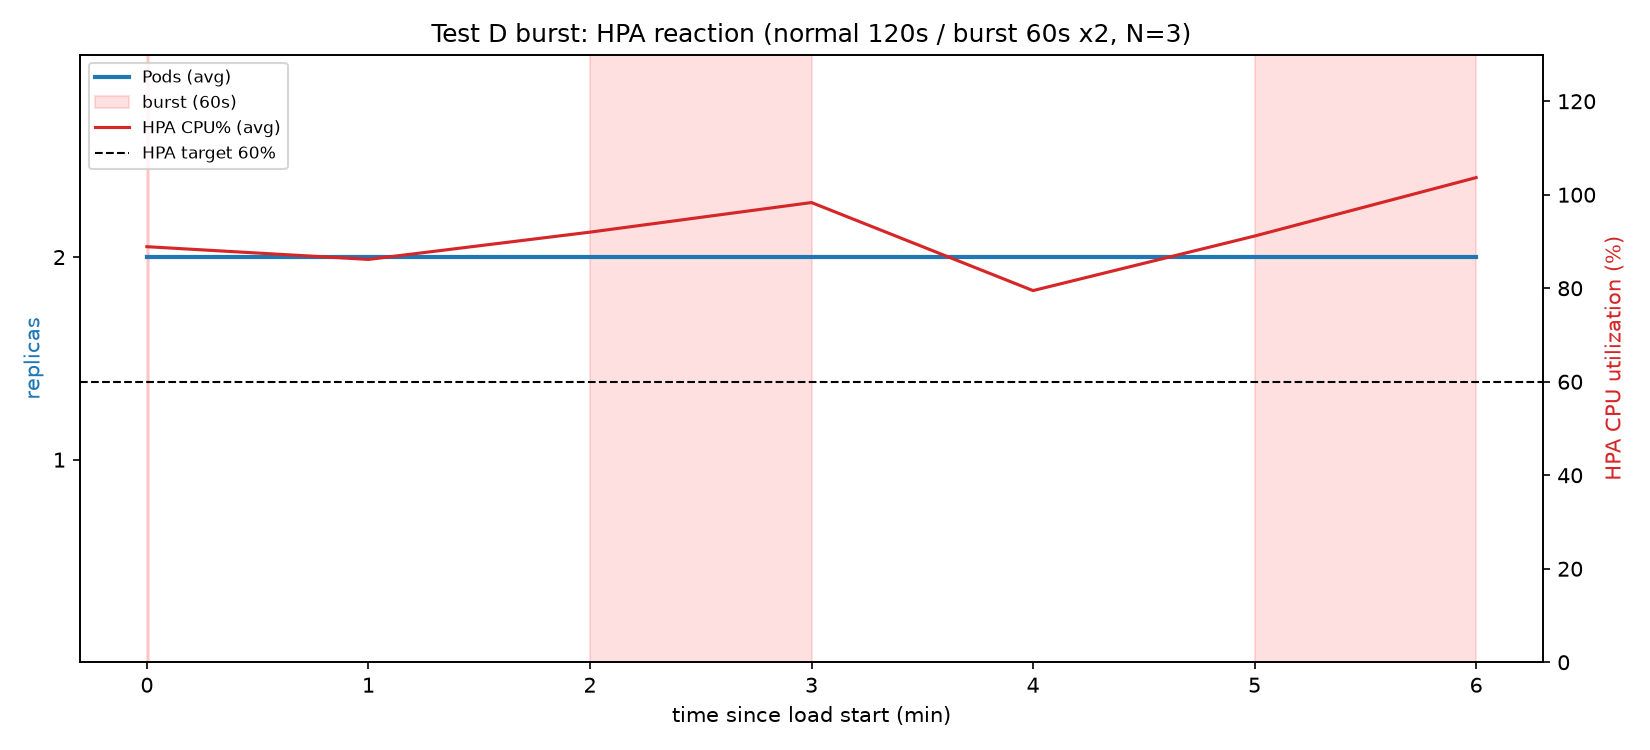
\includegraphics[width=\columnwidth]{figures/plot7_burst}
\caption{Test D: HPA reaction to bursts. CPU exceeds the 60\% target during
each burst and the HPA scales to two pods.}
\label{fig:burst}
\end{figure}

\subsection{Availability and SLO summary}
\label{sec:slasum}

Table~\ref{tab:sla} evaluates the objectives of Sec.~\ref{sec:sla}.

\begin{table}[t]
\caption{Compliance against the objectives stated in Sec.~\ref{sec:sla}}
\label{tab:sla}
\centering\small
\begin{tabular}{@{}llll@{}}
\toprule
Objective & Target & Measured & \\
\midrule
Elasticity scale-out & $\le$60 s & 0 s (Test A) & pass \\
Elasticity scale-in  & after valleys & every run, $\approx$224 s mean (Test A) & pass \\
Availability (2xx) @20u & $\ge$99\% & 98.8\% (Test C small) & pass \\
Error rate @20u      & $<$10\%  & 24\% (exp6 level 20) & \textbf{fail} \\
p95, small class     & $<$300 s  & 45.8 s (Test C) & pass \\
p95 @40--50 users    & $<$300 s  & 66--101 s (exp4/exp6) & pass \\
\bottomrule
\end{tabular}
\end{table}

The verdict is mixed in an informative way. Elasticity, the behaviour the
architecture exists to provide, passes cleanly in both directions. The
interactive latency and error objectives pass at design load and fail at
saturation, and the failure is the capacity ceiling (two pods) rather than the
autoscaler: with six pods (exp6) the same levels pass. The deployment is
correct and elastic; its ceiling is the number of workers.

\section{Cost Evaluation}
\label{sec:cost}

Per recommendation~R4 we project six months of operation and compare against
alternatives achieving the same objective. Every input is measured rather than
assumed (instance prices, 24/7 runtime; `r4\_cost.py`).

\subsection{Method}

The cluster runs continuously: 1 master \code{t3.small} (\$0.02/h) + 6 workers
\code{t3.medium} (\$0.042/h each) with a 40\,GB gp3 root volume each. We cost
three solutions for six months: (a) this stack with the HPA absorbing the
load; (b) a single \code{m5.4xlarge} (16 vCPU / 64\,GB, no elasticity) sized for
the same peak demand; (c) an equivalent AWS Lambda function (2\,GB memory,
40\,s mean invocation, 2.84M invocations per six months).

\subsection{Results}

\begin{table}[t]
\caption{Six-month cost projection}
\label{tab:cost}
\centering\small
\begin{tabular}{@{}lrr@{}}
\toprule
Solution & Compute & Total 6 mo \\
\midrule
K8s/EC2 stack (this project) & -- & \textbf{\$1{,}326.58} \\
Single m5.4xlarge (no autoscaling) & -- & \$4{,}226.88 \\
AWS Lambda (same AI app) & -- & \$3{,}787.24 \\
\bottomrule
\end{tabular}
\end{table}

The autoscaled cluster is cheapest (\$1{,}326.58; master \$106.86 + workers
\$1{,}219.73; the test-only load generator adds \$67.41). A single peak-sized
\code{m5.4xlarge} (16 vCPU, the same capacity as the six-worker fleet) costs
\$4{,}226.88, because without elasticity it runs at full size even when idle.
Lambda (\$3{,}787.24) sits in between, $\approx$2.9$\times$ the cluster: a long
CPU-bound inference is billed at serverless unit prices for every second of
decode, so a workload whose invocations last tens of seconds defeats the
serverless pricing model. The break-even duty cycle against a peak-sized
instance is well below 100\%, the HPA pays for itself whenever the service is
not saturated continuously.

The comparison is best read as a duty cycle, since that is the variable that
decides the architecture. At a fixed peak requirement (six workers) the
autoscaled cluster is \$1{,}327 only if it may scale down when idle; an
\code{m5.4xlarge} paid for six months is the cost of never scaling. The
serverless alternative is the mirror image: at low and bursty volumes Lambda
is competitive, but its unit cost per second of compute is so high that
sustaining ~0.2~req/s of LLM decode for six months ($\approx$3.1M seconds of
compute) reaches \$3{,}787. The crossing point is well below the utilisation a
production service would target, so for this workload, long, CPU-bound,
and always-on, provisioned elasticity wins. All prices are on-demand
us-east-1 list prices and exclude data transfer, which is identical across
solutions.

\section{Conclusion}

We evaluated a CPU-based HPA as the elasticity mechanism for an LLM inference
service on AWS Learner Lab, with a six-pod ceiling. Test~A drives the
deployment with a sawtooth profile and the HPA scales out $1{\to}2{\to}4{\to}6$
and back $6{\to}5{\to}4{\to}3{\to}2{\to}1$ in every one of $N{=}20$ runs,
including mid-run scale-\emph{in} with a mean latency of $\approx$224\,s, the
HPA stabilisation delay. Attributing
client wait time per request showed that llama decode accounts for the whole
latency budget while the orchestrator and transport contribute $\approx$11\,ms,
so the bottleneck is the model container, not Kubernetes.

The ceiling variant campaign asked whether the ceiling, not the autoscaler,
limits the service. Raising the HPA ceiling from four to six pods kept p95
below 100\,s and availability $\ge$0.76 at every level, and at level 50 the
six-pod deployment processed seven times the requests of the four-pod one by
absorbing the queue. Size isolation showed the cost of a request scales with
its length and that a mixed queue penalises short requests ~3.5\,$\times$. The
burst experiment showed the edge of the design: a sudden 6\,$\times$ step in
users is absorbed with zero errors across 145 requests because the queue
drains during the lull, while sustained load at the same intensity saturates
the queue.

Economically, the autoscaled cluster costs \$1{,}327 over six months against
\$4{,}227 for a peak-sized single instance and \$3{,}787 for the equivalent
Lambda deployment, so elasticity pays for itself and the CPU of an LLM service
is a sound scaling signal, provided the HPA ceiling is set to the worker count
the load actually needs. Measured against the objectives fixed in advance, the
deployment is elastic and correct; its limits are the number of workers and
the patience of the 300\,s timeout, not the autoscaler that decides how many
pods exist.

\begin{thebibliography}{9}\small
\bibitem{little} J. D. C. Little, ``A proof for the queuing formula
$L=\lambda W$,'' \emph{Operations Research}, vol.~9, no.~3, pp.~383--387, 1961.

\bibitem{adzic2017} G. Adzic and R. Chatley, ``Serverless computing: economic
and architectural impact,'' in \emph{Proc. 2017 11th Joint Meeting on
Foundations of Software Engineering (ESEC/FSE 2017)}, Paderborn, 2017,
pp.~884--889.

\bibitem{eivy2017} A. Eivy and J. Weinman, ``Be wary of the economics of
`serverless' cloud computing,'' \emph{IEEE Cloud Computing}, vol.~4, no.~2,
pp.~6--12, 2017.

\bibitem{llamacpp} G. Gerganov et al., \emph{llama.cpp} (open-source CPU LLM
inference engine), \url{https://github.com/ggml-org/llama.cpp}.

\bibitem{k8s} The Kubernetes Authors, \emph{Kubernetes Documentation:
Horizontal Pod Autoscaling},
\url{https://kubernetes.io/docs/tasks/run-application/horizontal-pod-autoscale/}.
\end{thebibliography}

\end{document}
